\documentclass[10pt]{article}

%\usepackage{arxiv}
% set page geometry
\usepackage[verbose=true,letterpaper]{geometry}
\AtBeginDocument{
	\newgeometry{
		textheight=9in,
		textwidth=6.5in,
		top=1in,
		headheight=14pt,
		headsep=25pt,
		footskip=30pt
	}
}

\usepackage[UTF8]{ctex}
\usepackage{amsmath}
\usepackage{authblk}
\usepackage{booktabs} 
\usepackage[]{algorithm2e}
\usepackage{algorithmic}
%\usepackage{blindtext}
\usepackage{times}
\usepackage{epsfig}
\usepackage{graphicx}
\usepackage{amssymb}
\usepackage{multirow}
% \usepackage[table]{xcolor}
\usepackage{subcaption}
\usepackage[pagebackref=true,breaklinks=true,letterpaper=true,colorlinks,bookmarks=false]{hyperref}

\newcommand{\qizhe}[1]{\textcolor{red}{#1}}
\newcommand{\qvl}[1]{\textcolor{red}{#1}}
\newcommand{\thang}[1]{\textcolor{blue}{#1}}

\def\ie{\emph{i.e}\onedot}
\def\eg{\emph{e.g}\onedot}


\makeatletter
\renewcommand\AB@affilsepx{\hspace{2pt}  \protect\Affilfont}
\makeatother

\title{“吵闹学生”自学法提高了ImageNet分类任务的成绩}

\author[1]{Qizhe Xie}
\author[2]{Eduard Hovy}
\author[1]{Minh-Thang Luong}
\author[1]{Quoc V. Le}

\affil[1]{Google Research, Brain Team}
\affil[2]{Carnegie Mellon University \protect\\}
\affil[ ]{\tt\small \{qizhex, thangluong, qvl\}@google.com, hovy@cmu.edu}

\renewcommand\Authands{, and }

\date{\small 2019年11月11日}

\hyphenation{Ima-ge-Net}
\hyphenation{Effi-cient-Net}

\begin{document}
\maketitle
\begin{abstract}
我们提出一个简单的自我训练模型。该模型在\-ImageNet数据库的分类中达到了87.4\%的第一准确率(top-1 accuracy)。这比先前的最优模型(该模型需要额外的350亿张来源于Instagram的弱标注图像作为补充训练集)高出了一个百分点。在健壮性训练集的测试中,我们的模型将\-ImageNet-A\-的第一准确率从16.6\%提高到了74.2\%,将\-ImageNet-C的平均损错误率(mean corruption error)从45.7降低到了31.2,将\-ImageNet-P的平均翻转率(mean flip rate)从27.8降低到了16.1。  


为了达到这一成果,我们首先利用已经标注的\-ImageNet图像训练了一个EfficientNet模型,并用这个模型作为“老师”来为3亿张没有标注的图像进行“假”标注。然后我们将一个更大的EfficientNet作为“学生”模型用已标注的和“假”标注的图像共同进行训练。这一过程可以迭代,也就是把新训练出来的“学生”模型变作“老师”,重复上述过程。在生成“假”标注的过程中不加入噪音,所以“假”标注会生成得尽可能准确。但是在“学生”模型学习的过程中,我们添加了噪音,比如数据扩增,随机丢弃(dropout),随机深度(stochastic depth),所以“学生”模型被强迫从“假”标注的图像中更加“努力”地获取有效信息。  
\end{abstract}

\section{背景介绍}

近些年来,深度学习在图像识别邻域取得了非凡地成功
~\cite{krizhevsky2012imagenet, szegedy2015going, simonyan2014very, he2016deep, tan2019efficientnet}。但是,最优的模型依然需要庞大数量的已标注图像作为语料库来进行监督学习。这也就限制了我们使用更加庞大数量的未标注图像来提高最优模型的准确度和健壮性的能力。  


在本文中,我们利用未标注图像提高了最优模型在ImageNet分类上的准确度,并展示出这种准确度的提升同时对模型健壮性的提高也有巨大的帮助。为达到这一目的,我们使用了大量的未标注图像,甚至有些图像并不属于ImageNet中的任何一类。我们使用自我训练(self-training)方法~\cite{scudder1965probability}。这一方法包含三个主要步骤: 1)用已标注图像训练一个“老师”模型,2)用这个“老师”模型来标注未标注的图像,从而产生“假”标注,3)用已标注和“假”标注的图像共同训练“学生”模型。最后,我们把上述过程迭代多次,把训练好的“学生”模型作为“老师”来标注更多的未标注图像,然后训练新的“学生”模型。  


在我们实验的过程中发现,使得这一简单方法工作的关键因素是:在训练“学生”的时候需要在训练集中加入噪音,而在“老师”模型生成“假”标注的时候不应当加入噪音。这样,产生的“假”标注会尽可能的准确,同时“学生”会更加“努力”地学习“假”标注提供的额外信息。为了给“学生”学习的过程中加入噪音,我们使用了随机丢弃\cite{srivastava2014dropout},数据扩增~\cite{cubuk2019RandAugment},随机深度~\cite{huang2016deep}的方法。我们把这种方法称作“吵闹学生”自学法以凸显噪音在训练过程和提高最终结果中所扮演的重要角色。为了在ImageNet分类任务中得到很好的结果,“学生”模型需要很大,比一般意义上的计算机视觉模型更大,才能平衡大量的未标注图像带来的信息增加。  


使用“吵闹学生”自学法以及3亿张未标注的图像,我们把\-EfficientNet~\cite{tan2019efficientnet}\-在\-ImageNet\-分类任务中的第一准确率提高到了87.4\%.这一准确率比先前的最优模型高出1\%.而且,先前的最优模型需要35亿张弱标注(weakly labeled)的来源于Instagram的图片进行训练。我们的模型不仅提高了\-ImageNet\-分类的准确度,也大幅提高了健壮性。在更加困难的\-ImageNet-A~\cite{hendrycks2019natural}\-数据中,分类第一准确度从16.6\%提高到了74.2\%,ImageNet-C~\cite{hendrycks2018benchmarking}的平均损错误率(mean corruption error, mCE)从45.7降低到了31.2,ImageNet-P~\cite{hendrycks2018benchmarking}的平均反转率从27.8降低到了16.1。表~\ref{tab:summary}展示了我们的主要结果。

\begin{table}[h!]
	\footnotesize
	\centering 
	\begin{tabular}{l|cccc}           
		\toprule 
		&  ImageNet & ImageNet-A & ImageNet-C & ImageNet-P \\
		&  top-1 acc. & top-1 acc. & mCE & mFR \\
		\midrule      
		
		Prev. SOTA  & 86.4\% & 16.6\% & 45.7 & 27.8\\  % Previous state-of-art
		Ours & \bf 87.4\% & \bf 74.2\% & \bf 31.2 & \bf 16.1\\ % ST with Noisy Student
		\bottomrule
	\end{tabular}
	\caption{关键结果总结和与先前最优模型的比较~\cite{touvron2019fixing,mahajan2018exploring}. 平均损错误率和平均翻转率越低越好。}  
	\label{tab:summary}
\end{table}

\section{“吵闹学生”自学法模型}
算法~\ref{algo:noisy_student}给出了“吵闹学生”自学法的概览。我们用已标注的图像作为输入,交叉熵(cross entropy)作为损失函数训练一个“老师”模型。然后用这个“老师”模型生成未标注图像的“假”标注。“假”标注可以是软性的(连续分布)或者硬性的(单激活(one-hot)分布)。接着我们通过同时最小化在已标注和“假”标注图像上的交叉熵来训练一个“学生”模型。最后,迭代这一过程,把训练好的“学生”放回到“老师”的位置上,产生更多的“假”标注,再训练新的学生。

\begin{algorithm}
	\small
	\caption{“吵闹学生”模型}
	\label{algo:noisy_student}
	\begin{algorithmic}[1]
		\REQUIRE 
		已标注图像 $\{(x_1, y_1), (x_2, y_2), ..., (x_n, y_n)\}$ 和未标注图像 $\{\tilde{x}_1, \tilde{x}_2, ..., \tilde{x}_m\}$.
		\STATE  通过最小化在已标注模型上的交叉熵来训练“老师”模型 $\theta_{*}$  $$\frac{1}{n}\sum_{i = 1}^n \ell(y_i, f^{noised}(x_i, \theta) )$$ \\ 
		\STATE 用没有加入噪音的“老师”模型为未标注图像生成“假”标注 $$\tilde{y}_i = f(\tilde{x}_i, \theta_{*}), \forall i = 1, \cdots, m $$ \\
		\STATE 通过最小化在加入了噪音的已标注和“假”标注的图像上的交叉熵来训练“学生”模型 $\theta_*'$ $$\frac{1}{n}\sum_{i=1}^n \ell(y_i, f^{noised}(x_i, \theta') ) + \frac{1}{m} \sum_{i=1}^m \ell (\tilde{y}_i, f^{noised}(\tilde{x}_i, \theta')) $$\\
		\STATE 迭代训练:“学生”变“老师”,回到步骤2.
		
	\end{algorithmic}
\end{algorithm}

这一算法基本上是自我训练,半监督式学习的方法(例如,~\cite{scudder1965probability,yarowsky1995unsupervised})。我们会在第五部分讨论这一工作和先前工作之间的联系。主要的改变是给“学生”模型增加了更多不同种类的噪音的同时去除了“老师”模型在产生“假”标注过程中的的噪音。  


当我们故意加入噪音来训练“学生”模型的时候,它会恒定地接近更加准确地,没有被噪音影响地“老师”模型。在我们的实验中,使用了随机丢弃\cite{srivastava2014dropout},随机深度~\cite{huang2016deep},数据扩增~\cite{cubuk2019RandAugment},来给“学生”添加噪音。  


尽管噪音听起来很无趣,但是当把它加运用到未标注的图像上时,会产生一种有益的复合效应。它会使训练出来的模型无论在对已标注的还是未标注的图像分类时,都具有更平顺(smoothness)的决定函数(decision function)。不同种类的噪音可能具有不同的效果。在使用数据扩增时,训练出来的“学生”模型必须保证平移前后的图像被分入同一类。这种限制降低了模型的自由度。当采用随机丢弃和随机深度时,训练出来的“学生”模型再作为“老师”时,更像是多个模型的组合(ensemble of models)(生成“假”标注时,没有使用随机丢弃),而它的“学生”是一个单一模型。换而言之,“学生”是在向一个更加强大的组合模型学习。  


“学生”和“老师”模型的架构可以相同也可以不同。但是,为了使“吵闹学生”模型可以良好工作,“学生”模型须要足够大,以容纳更多的数据(已标注和“假”标注)。为达到这一目的,我们用最近开发的EfficientNet~\cite{tan2019efficientnet}架构因为它具有比ResNet~\cite{he2016deep}更大的容量。其次,为了让“学生”更加强大,我们让“学生”的模型比“老师”大。这是我们的工作和先前工作的一个重要差异。先前的工作使用“老师”-“学生”构造的主要目的是压缩模型的大小。  


我们还发现另一个窍门可以让“吵闹学生”模型工作得更好:平衡数据。具体来说,因为ImageNet数据库中各类图像的数量大致相当,我们同样需要平衡未标注图像的数量。对于图像数量比较少的类,我们采取复制的办法。对于图像数量比较多的类,我们只取质量最好的图像。  


最后,在前文中我们提到,“假”标注可以是软性的也可以是硬性的。在实际操作过程中我们观察到使用软性标注往往使训练更加稳定并且收敛得更快。尤其是“老师”模型本身得准确度比较低时。所以,除非特别说明,我们都采用软性标注进行实验。  

\section{实验}
接下来,我们首先介绍可以得到我们实验结果的实验细节。接着展示在ImageNet分类任务中我们的模型和先前最优模型的比较。最后我们会展示在健壮性基准数据集上,例如ImageNet-A,C和P,我们的模型的表现以及对抗健壮性(adversarial robustness)。  

\subsection{实验细节}

\paragraph{已标注数据集 }
我们的实验是在2012 ILSVRC分类预测挑战的ImageNet数据集上进行的。因为这一数据集已经成为当下计算机视觉邻域使用最多的基准数据集,并且,普遍认同,在这一数据集上的提高可以转移到其它数据上~\cite{kornblith2019better,recht2019imagenet}。 

\paragraph{未标注数据集}
我们的未标注图像是从JFT数据集~\cite{hinton2015distilling, chollet2017xception}中获取的。这个数据集拥有大约3亿张图片。尽管这些图片有标注,我们忽略它们的标注,把它们当作未标注图像来使用。我们使用的版本来自~\cite{ngiam2018domain},ImageNet的验证集已经从这个版本中剔除。  


在获取了这些图像后,我们进行了过滤和平衡。首先,我们用一个在ImageNet上训练过的EfficientNet-B0~\cite{tan2019efficientnet}为JFT的每一幅图像预测一个标注。接着我们选择出预测标注的自信度在0.3以上的图像。每一类的图像数量不超过13万幅。如果数量多于13万,我们优先选择自信度高的图像。最后,对于图像数量少于13万的类,我们随机复制一部分图像,使得每一类的图像数量都是13万。因此,总共用来训练“学生”的图像数量是1.3亿(包括复制的图像)。因为复制,在这1.3亿幅图像中只有8千万独一无二的图像。我们没有进一步调校这些参数,因为我们的模型在这些参数条件下已经表现出非常好的健壮性。  

\paragraph{架构}
因为容量大,我们选择EfficientNet~\cite{tan2019efficientnet}作为我们的基线模型。在实验过程中,我们进一步加大了EfficientNet-B7,得到了EfficientNet-L0,L1和L2。EfficientNet-L0比EfficientNet-B7更深更宽,但是分辨率较低。这使得它有更多的参数来容纳更多的未标注图像的同时具有和EfficientNet-B7类似的训练速度。EfficientNet-L1是在EfficientNet-L0的基础上进一步加宽。最后,我们根据符合缩放(compound scaling~\cite{tan2019efficientnet})的方法在所有维度上扩大而得到了EfficientNet-L2。因为模型巨大,EfficientNet-L2的训练时间几乎是EfficientNet-B2的5倍。更多信息请参照附录\ref{sec:architecture_details}表\ref{tab:efficientnet_architectures}。  

\paragraph{训练细节}
对于已标注图像,我们使用2048的批容(batch size)。当内存无法容纳模型的时候,我们再逐步减小批容。我们发现,使用512,1024,2048的批容所得到的结果是一致的。我们根据批容决定训练的总步数(training steps)和学习速率(learning rate)。具体来说,当“学生”模型大于EfficientNet-B4的时候,我们进行350轮(epoch)训练,其中包括了EfficientNet-L0,L1和L2。对其余较小的模型,进行700轮训练。起始训练速率为0.128,衰减率0.97每2.4轮如果进行350轮训练。如果进行700轮训练,每4.8轮进行一次衰减。  


对未标注图像,对于EfficientNet-B7,L0,L1和L2这样的大模型,我们使用三倍于已标注图像的批容。对小模型,我们使用和已标注图像一样的批容。在代码实现中,已标注和未标注的图像被连接(concatenate)在一起,计算平均交叉熵损失。


最后,我们运用最近刚提出的技术来锁定EfficientNet-L0,L1和L2在训练和测试之间的分辨率差异~\cite{touvron2019fixing}。具体来说,我们首先用比较小的分辨率训练350轮。之后我们用没有经过扩增已标注图像和较大的分辨率对模型进行优化。和\cite{touvron2019fixing}类似,我们在优化时锁定了较浅的层(shallow layers)。  


我们最大的模型,EfficientNet-L2,需要在2048核的Cloud TPU v3 Pod上训练3.5天。

\paragraph{噪音}
我们采用随机深度~\cite{huang2016deep},随机丢弃\cite{srivastava2014dropout},数据扩增~\cite{cubuk2019RandAugment}来给“学生”引入噪音。在EfficientNet-B7,L0,L1和L2中,噪音函数的高级参数(hyperparameters)保持不变。具体来说,我们将最后一层的随机深度的生存几率(survival probability)设置为0.8,其余各层线性递减。我们为最后的分类层设置了0.5的随机丢弃机率。对随机数据扩增(这里使用了RandAugment),我们进行了两项随机操作,尺度(magnitude)设置为27。

\paragraph{迭代训练}
我们实验中最好的模型是将受过训练的“学生”放回到老师的位置来产生新的“假”标注的迭代方法。在此过程中,我们不断提高“学生”模型的大小来提高准确度。过程如下:我们首先使用EfficentNet-B7同时作为“老师”和“学生”来提高EfficientNet-B7的准确度。接着用提高过的EfficientNet-B7作为“老师”训练EfficientNet-L0。然后用EfficientNet-L0作为“老师”训练EfficientNet-L1。接着用EfficientNet-L1训练EfficientNet-L2.最后用EfficientNet-L2作为老师训练另外一个EfficientNet-L2。

\begin{table*}[h!]
	\small
	\centering      
	\begin{tabular}{l|cc|cc}                                                
		\toprule 
		模型 & \ 参数数量 & 额外数据  &  第一准确率  &  前五准确率   \\
		\midrule       
		ResNet-50 \cite{he2016deep} & 26M & -  & 76.0\% & 93.0\%   \\
		ResNet-152 \cite{he2016deep} & 60M  & - &  77.8\% & 93.8\% \\
		DenseNet-264 \cite{huang2017densely} & 34M & - & 77.9\% & 93.9\%   \\
		Inception-v3 \cite{szegedy2016rethinking}& 24M  & - & 78.8\% & 94.4\%  \\
		Xception \cite{chollet2017xception} & 23M & - & 79.0\%   & 94.5\%  \\
		Inception-v4 \cite{szegedy2017inception} & 48M  & - & 80.0\% & 95.0\%  \\  
		Inception-resnet-v2  \cite{szegedy2017inception} & 56M & - & 80.1\% & 95.1\% \\  
		ResNeXt-101 \cite{xie2017aggregated}  & 84M   & - & 80.9\% & 95.6\% \\
		PolyNet \cite{zhang2017polynet}  & 92M  & - & 81.3\%  & 95.8\% \\
		SENet \cite{hu2018squeeze} & 146M & - & 82.7\% & 96.2\%   \\
		NASNet-A \cite{zoph2018learning} & 89M & - & 82.7\% & 96.2\%   \\
		AmoebaNet-A \cite{real2019regularized} & 87M & - & 82.8\% & 96.1\%   \\
		PNASNet \cite{liu2018progressive} & 86M  & - & 82.9\% & 96.2\%  \\
		AmoebaNet-C  \cite{cubuk2018autoaugment}  & 155M  & - &  83.5\%  & 96.5\% \\
		GPipe \cite{gpipe18} & 557M & - & 84.3\%  & 97.0\%   \\
		EfficientNet-B7 \cite{tan2019efficientnet} &  66M  & - & 85.0\% & 97.2\%   \\
		EfficientNet-L2 \cite{tan2019efficientnet} &  480M  & - & 85.5\% & 97.5\%   \\
		\midrule
		ResNet-50 Billion-scale \cite{billion_large_scale} & 26M & \multirow{4}{*}{3.5B images labeled with tags} & 81.2\% & 96.0\% \\
		ResNeXt-101 Billion-scale \cite{billion_large_scale} & 193M &  & 84.8\% & - \\
		ResNeXt-101 WSL \cite{mahajan2018exploring} & 829M &   & 85.4\% & 97.6\% \\
		FixRes ResNeXt-101 WSL \cite{touvron2019fixing} & 829M  &  & 86.4\% &  98.0\%  \\
		\midrule
		\bf Noisy Student (L2) &  480M & 300M unlabeled images & \bf 87.4\% & \bf 98.2\%  \\
		\bottomrule
	\end{tabular}
	\caption{“吵闹学生”法和先前最优方法在ImageNet任务中的第一和前五准确率。“吵闹学生”法训练的EfficientNets在准确率和模型大小之间取得了更好的平衡。表中的Noisy Student (L2)是用迭代训练法迭代多次后的结果。}  
	\label{tab:imagenet}
\end{table*}

\subsection{ImageNet分类结果}
按常规~\cite{krizhevsky2012imagenet,szegedy2015going,he2016deep,tan2019efficientnet} (还有 \cite{recht2019imagenet}),我们首先报告在ImageNet 2012 ILSVRC分类预测挑战中的成绩。结果如表\ref{tab:imagenet},用“吵闹学生”法训练的EfficientNet-L2模型能够达到87.4\%的第一准确率,比先前EfficientNet的85.0\%有显著提高。提高的2.4\%源自两个方面:模型更大(+0.5\%),“吵闹学生”法(+1.9\%).换句话说,使用“吵闹学生”算法对准确度的提升大于更换模型的提升。  


“吵闹学生”同样超过先前最优模型FixRes ResneXt-101 WSL~\cite{mahajan2018exploring,touvron2019fixing}的86.4\%准确率。相比较FixRes ResneXt-101 WSL 来源于Instagram的35亿的已标注训练集,我们的模型仅仅需要3亿未标注的图像作为训练集。这种训练集更容易收集到。我们的模型的参数数量也比FixRes ResneXt-101 WSL少了接近一半。  

\begin{figure}[h!]
	\centering
	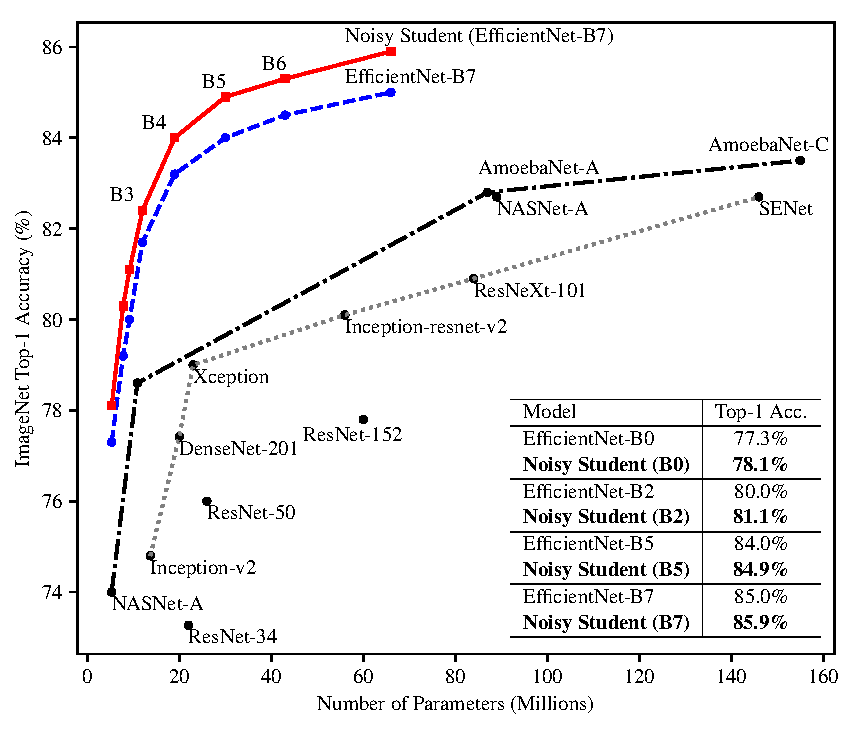
\includegraphics[width=\columnwidth]{fig/plot_vary_model_size.pdf}
	\caption{“吵闹学生”法显著提高了所有大小的EfficientNet的成绩。“老师”和“学生”使用的是同样的架构。在这个实验中我们没有使用迭代训练。}
	\label{fig:vary_model_size}
\end{figure}

\paragraph{模型大小研究:不用迭代训练的“吵闹学生”(EfficientNet B0-B7)}
除了提高最优结果,我们进一步实验证明了“吵闹学生”法可以惠及其它的EfficientNet模型。在前面的实验中,我们用迭代训练的方式有化EfficientNet-L2.这里我们放弃这一方法,因为在大量测试中,很难每次都采用迭代训练的方法。我们使用EfficientNet-B0到B7~\cite{tan2019efficientnet},在每次实验中用一样的模型同时做老师和学生.我们在训练所有EfficientNet基线模型的时候都引入了数据扩增,这使得这些基线模型更具有竞争力。如图\ref{fig:vary_model_size}所示,在所有模型中,“吵闹学生”稳定地保持约0.8\%的领先。总的来说,使用“吵闹学生”法训练的EfficientNet模型在模型大小和准确率之间找到了更好的平衡点。这些结果也肯定了,即使不使用多次迭代,视觉模型也可以从“吵闹学生”方法中获益。

\subsection{在ImageNet-A,ImageNet-B和ImageNet-C上健壮性的测试结果}
我们评估了达到87.4\%第一准确率的最佳模型在三个健壮性模型,ImageNet-A,ImageNet-C和ImageNet-P,上的表现。ImageNet-C和ImageNet-P中的图片有常见的损毁,比如模糊,雾化,旋转和缩放。ImageNet-A由一些先前最优模型都难以进行分类预测的图片组成。这些数据集之所以被称为健壮性测试基准集,是因为它们要么非常困难,如ImageNet-A,要么训练集和测试集有差别,如ImageNet-C和P.  


对ImageNet-C和ImageNet-P,我们使用了两个已经发布的版本,分辨率分别为224x224和299x299.这些图片被拉伸到了EfficientNet训练集的大小。  

\begin{table}[h!]
	\small
	\centering 
	\begin{tabular}{l|ccc}                                                
		\toprule 
		Method &  Top-1 Acc. & Top-5 Acc. \\
		\midrule      
		ResNet-101~\cite{hendrycks2019natural} & 4.7\% & - \\
		ResNeXt-101~\cite{hendrycks2019natural} (32x4d) & 5.9\% & -  \\
		ResNet-152~\cite{hendrycks2019natural} & 6.1\% & - \\
		ResNeXt-101~\cite{hendrycks2019natural} (64x4d) & 7.3\% & - \\
		DPN-98~\cite{hendrycks2019natural} & 9.4\% & - \\
		ResNeXt-101+SE~\cite{hendrycks2019natural} (32x4d) &  14.2\% & - \\
		ResNeXt-101 WSL~\cite{mahajan2018exploring,orhan2019robustness} & 16.6\% & - \\
		\midrule
		EfficientNet-L2  &  49.6\% & 78.6\%   \\
		\bf Noisy Student (L2) & \bf 74.2\% & \bf 91.3\%  \\
		\bottomrule
	\end{tabular}
	\caption{ImageNet-A的健壮性测试结果}  
	\label{tab:robustness1}
\end{table}


\begin{table}[h!]
	\small
	\centering 
	\begin{tabular}{l|c|cc}         
		\toprule 
		Method & Res. & Top-1 Acc. & mCE \\
		\midrule
		ResNet-50 \cite{hendrycks2018benchmarking} & 224 & 39.0\% & 76.7 \\
		SIN \cite{geirhos2018imagenet} &224 & 45.2\% & 69.3 \\
		Patch Guassian \cite{lopes2019improving}  & 299 & 52.3\% & 60.4 \\
		ResNeXt-101 WSL~\cite{mahajan2018exploring,orhan2019robustness} & 224 & - & 45.7 \\
		\midrule
		EfficientNet-L2  & 224 &  62.6\% &  47.5 \\
		Noisy Student (L2) & 224  &  72.8\% &  34.7 \\
		
		EfficientNet-L2  & 299 & 66.6\% & 42.5  \\
		\bf Noisy Student (L2) & 299 & \bf 75.5\% & \bf 31.2 \\
		\bottomrule
	\end{tabular}
	\caption{ImageNet-C的健壮性测试结果. mCE(平均损毁错误率)是不同损毁方式中错误率的甲醛平均,以AlexNet的错误率为基线。(越低越好)}  
	\label{tab:robustness2}
\end{table}

\begin{table}[h!]
	\small
	\centering
	\begin{tabular}{l|c|cc}         
		\toprule 
		Method & Res. & Top-1 Acc. & mFR \\
		\midrule
		ResNet-50 \cite{hendrycks2018benchmarking} & 224 & - & 58.0 \\
		Low Pass Filter Pooling \cite{zhang2019making} &224 & - & 51.2 \\
		
		ResNeXt-101 WSL~\cite{mahajan2018exploring,orhan2019robustness} & 224 & - & 27.8  \\
		\midrule
		EfficientNet-L2  & 224 & 80.4\% & 27.2  \\
		Noisy Student (L2) & 224 &  83.1\% & 17.8  \\
		EfficientNet-L2  & 299 & 81.6\% &  23.7 \\
		\bf Noisy Student (L2) & 299 & \bf 84.3\% & \bf 16.1 \\
		\bottomrule
	\end{tabular}
	\caption{ImageNet-P的健壮性测试结果。 图像由一系列的干扰产生。mFR(平均翻转率)是指模型在干扰下改变预测的机率,以AlexNet为基线。(越低越好)}  
	\label{tab:robustness3}
\end{table}

如表\ref{tab:robustness1},表\ref{tab:robustness2} 和表\ref{tab:robustness3}所示,在和先前的最优模型ResNeXt-101 WSL~\cite{mahajan2018exploring,orhan2019robustness}的比较中,“吵闹学生”在健壮性上显示出了绝对的提升。在ImageNet-C中,它把平均损错误率(mCE)从45.7降低到了31.2。在ImageNet-P中,如果使用224x224的分辨率,它可以达到17.8的平均翻转率。如果用299x299\footnote{For EfficientNet-L2, we use the model without finetuning with a larger test time resolution, since a larger resolution results in a discrepancy with the resolution of data and leads to degraded performance on ImageNet-C and ImageNet-P.}的分辨率,这一数值将提高到16.1。这些在健壮性上的显著提升是在预料之外的,因为我们并没有专门对模型进行健壮性上的优化(比如通过数据扩增)。  


最大的提升是在ImageNet-A的结果中观察到的:我们的模型获得了3.5倍的准确率提升。第一准确率从先前的最优结果16.6\%提高到了74.2\%.相对应的,改变模型或者使用弱标注的数据进行训练,仅仅能够把准确率从4.7\%提高到了16.6\%.

\paragraph{定性分析}
为了能够从直觉上理解在健壮性基准集上准确率的显著提升,我们在图\ref{fig:robustnessacp}中展示了几张图像。基准模型在这些图像上的预测结果是错误的,而“吵闹学生”可以对这些图像做出正确预测。  


图\ref{fig:imagenet_a}中为来自ImageNet-A的示例图像和我们的模型给出的预测结果。“吵闹”学生模型可以成功预测这些困难图片的标注。例如,在不使用“吵闹学生”的情况下,模型对第二行左侧的图片给出的标注是牛蛙,这有可能是因为水里黑色的睡莲叶子导致的误判。使用了“吵闹学生”后,模型正确地把这幅图像标注为蜻蜓。在左上角地图像中,不使用“吵闹学生”的模型忽略了海狮并且错误地将浮标认成了灯塔,而使用了“吵闹学生”的模型可以正确认出海狮。  


图\ref{fig:imagenet_c}中展示了来自ImageNet-C的图像和相应的预测结果。从图中可以看出,对于被比如雪、动态模糊、雾严重损坏和干扰的图像,我们的“吵闹学生”模型依然可以给出正确的预测。而没有使用“吵闹学生”的模型在这些情况下遭遇了严重困难。最有趣的是右上角的那幅图,图像中的秋千连人类都很难认出,但是“吵闹学生”依旧给出了正确的预测。  


图\ref{fig:imagenet_p}中的是ImageNet-P的图像和相应的预测。可以看出,在图片受到不同的干扰时,我们的“吵闹学生”模型依旧稳定地给出正确地预测。没有使用“吵闹学生”的模型频繁地转换预测结果。比如,右边的一列,在图像中的车被轻微旋转的过程中,基准模型给出了赛车,车轮,消防车等不同预测。相对的,我们的“吵闹学生”模型可以保持稳定。  

\begin{figure*}[!htb]
	\begin{subfigure}{.33\textwidth}
		\centering
		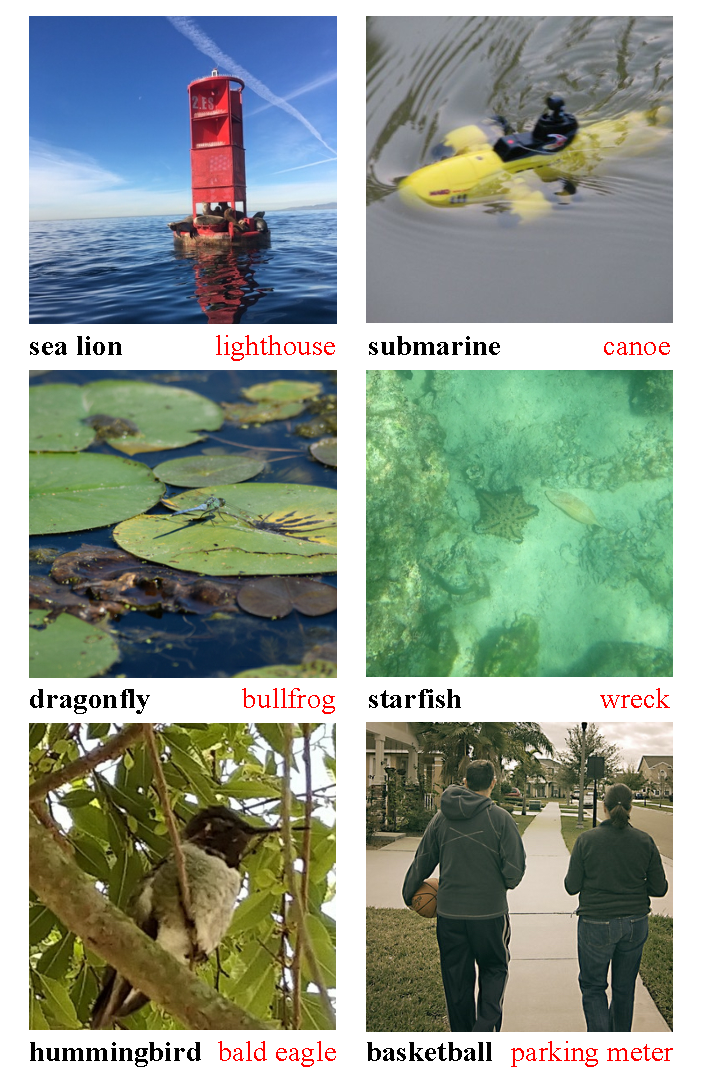
\includegraphics[width=\linewidth]{fig/imagenet_a}
		\caption{ImageNet-A}
		\label{fig:imagenet_a}
	\end{subfigure}\hfill
	\begin{subfigure}{.33\textwidth}
		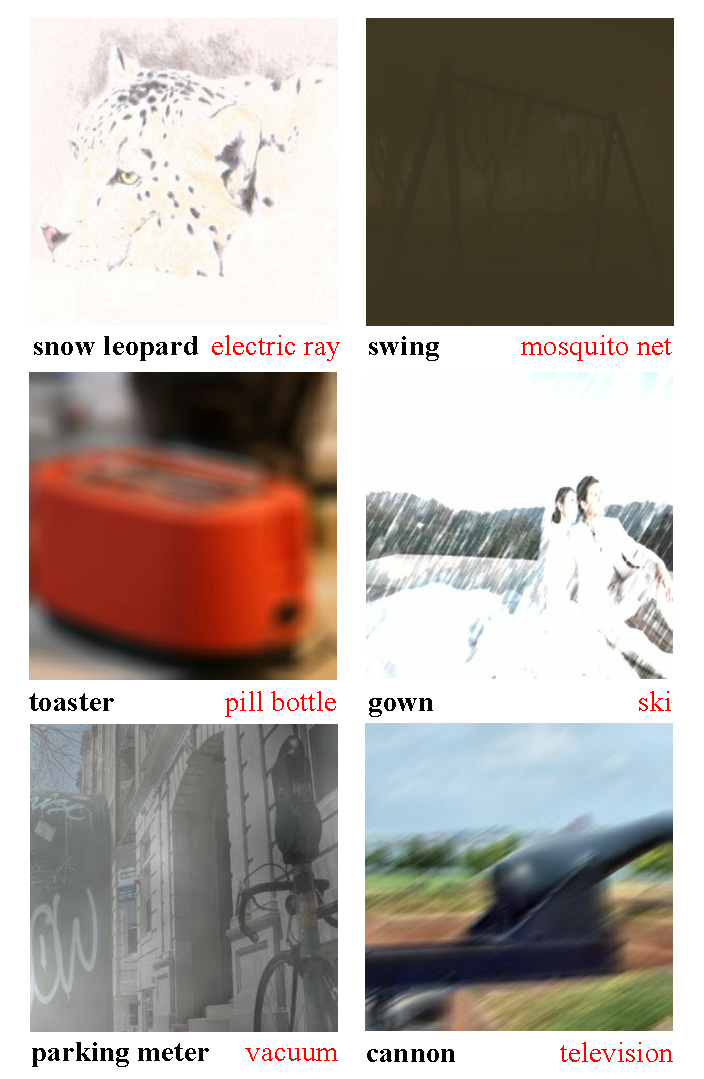
\includegraphics[width=\linewidth]{fig/imagenet_c}
		\caption{ImageNet-C}
		\label{fig:imagenet_c}
	\end{subfigure}\hfill
	\begin{subfigure}{.33\textwidth}
		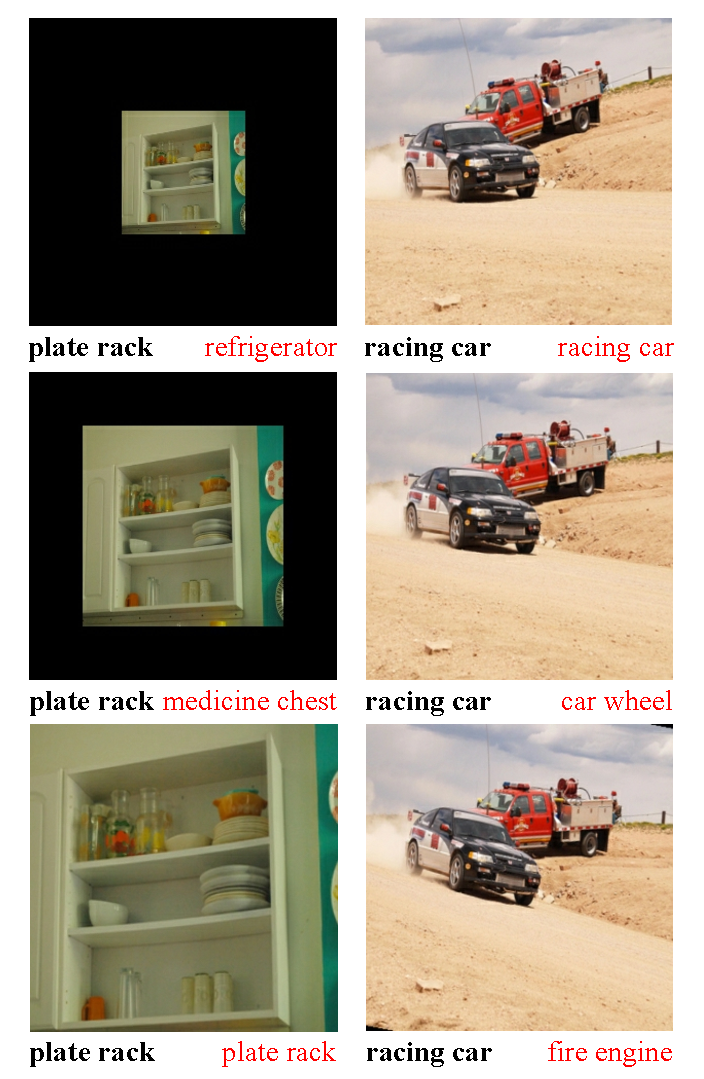
\includegraphics[width=\linewidth]{fig/imagenet_p}
		\caption{ImageNet-P}
		\label{fig:imagenet_p}
	\end{subfigure}\hfill
	\caption{从ImageNet-A,C和P中挑选的图像。ImageNet-C中的测试图像已经从ImageNet训练集中排除。ImageNet-P中的测试图片经过了不同幅度的干扰。经“吵闹学生”法训练的EfficientNet做出正确的预测(\textbf{粗体}字),而未经“吵闹学生”法训练的EfficientNet在ImageNet-A和C中做出错误的预测,并频繁改变在ImageNet-P中的预测结果(\textcolor{red}{红色}字体)}
	\label{fig:robustnessacp}
\end{figure*}

\subsection{对抗健壮性(adversarial robustness)结果}
经过一般损毁和干扰测试之后,我们还对我们的模型进行了对抗性干扰测试。我们对使用了和没使用“吵闹学生”的EfficientNet-L2进行了快速梯度方向法(Fast Gradient Sign Method, FGSM)攻击,并对结果做了评测。快速梯度方向法指的是对原始图片的每一个像素做一次梯度下降\cite{goodfellow2014explaining},方向为梯度方向,步长为$\epsilon$.如图\ref{fig:adv_robustness}所示,虽然“吵闹学生”没有针对对抗健壮性进行优化,它依然带来了约10\%的准确率提升。  


我们之所以没有拿对抗健壮性的结果与以前的工作进行直接对比,是因为我们使用了800x800的较大的输入分辨率,而对抗脆弱性(adversarial vulnerability)会随着输入尺寸的变化而变化\cite{galloway2019batch,goodfellow2014explaining,gilmer2018adversarial,simon2019first}。可能以为同样的原因,当$\epsilon=16$时,EfficientNet-L2在10轮迭代的映射梯度下降(projected gradient descent, PGD)\cite{madry2017towards}的强攻击下准确率仅有1.1\%,远远落后于最优模型。“吵闹学生”能够把准确度提高到1.6\%. 

\begin{figure}[h!]
	\centering
	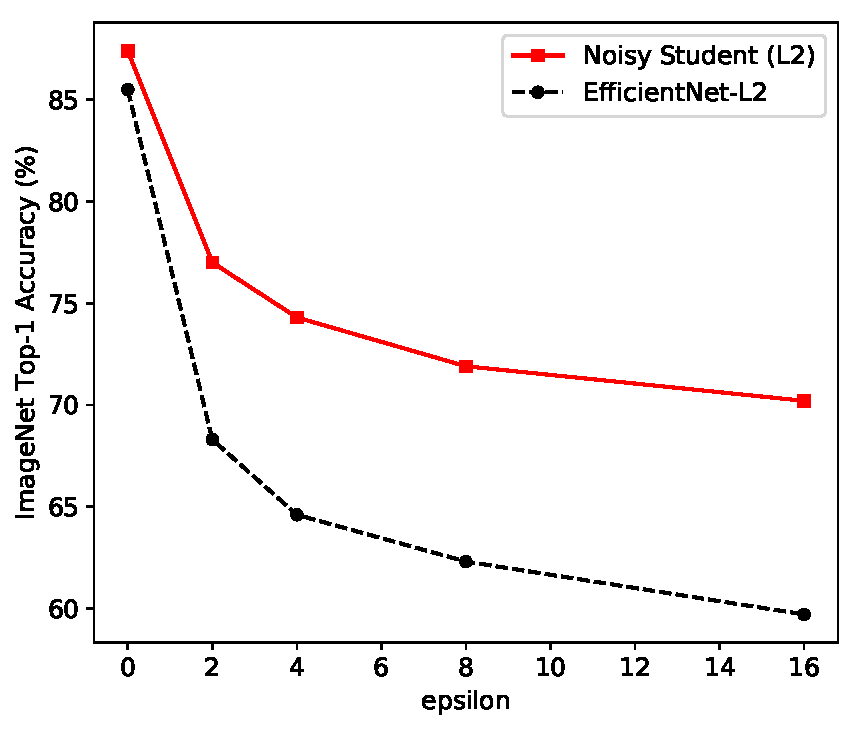
\includegraphics[width=0.9\columnwidth]{fig/plot_adv}
	\caption{“吵闹学生”提高了对抗FGSM攻击的健壮性,尽管模型并没有针对对抗健壮性进行优化。在多数设置下,准确率提高了10\%.实验中使用的是800x800的分辨率。}
	\label{fig:adv_robustness}
	
\end{figure}

\section{切除实验:自我训练中噪音的重要性}
在这一章节中,我们研究噪音的重要性,以及我们使用的几种噪音的不同效果。因为我们采用了“老师”模型生成的软性“假”标注,如果把“学生”训练成和“老师”完全一样的模型,那么在未标注的图像上的交叉熵损失将会变为0,训练信号(training signal)也会消失。因此,一个自然而然地问题就是,为什么“学生”会比“老师”优秀?正像前文中提到过的,我们假设给“学生”添加噪音是必须的,这样“学生”才不会仅仅学习到“老师”的知识。我们调查了不同未标注图像数量和不同“老师”模型准确率这两种情况下噪音的重要性。在两种情况中,我们都逐步移除对未标注图像的数据扩增、随机深度和随机丢弃,但是保持已标注图像的操作不变。这样我们就能把噪音对未标注图像的影响分离出来,而不会和防止对已标注图像的过拟合效应相混淆。  

\begin{table}[h!]
	\small
	\centering                                                                 
	\begin{tabular}{l|cc}                                                
		\toprule 
		Model / Unlabeled Set Size &    1.3M & 130M  \\
		\midrule      
		EfficientNet-B5  & 83.3\% & 84.0\% \\
		\midrule
		Noisy Student (B5) & \bf 83.9\% & \bf 84.9\% \\
		\  w/o Aug & 83.6\% & 84.6\% \\
		\  w/o Aug, SD, Dropout & 83.2\% & 84.3\% \\
		\bottomrule
	\end{tabular}
	\caption{针对噪音的效果进行的切除实验。我们用EfficientNet-B5同时作为“老师”和“学生”模型,研究了不同未标注图像数量和不同数据扩增方法下的两种情形。在130万幅图像的情况下,我们用了随机移位和选装的标准数据扩增方法。在1.3亿幅图像的情况下,我们使用了RandAugment. Aug和SD分别表示数据扩增和随机深度。我们移除了未标注图像的噪音,而保留了已标注图像的噪音。为了简化,在此实验中我们没有使用迭代训练。}
	\label{tab:abl_noise}
\end{table}

表\ref{tab:abl_noise}中列出的证据证明,例如数据扩增、随机深度和随机丢弃这样的噪音对“学生”超越“老师”起着至关重要的作用。在逐步移除噪音函数的过程中,模型的表现稳定下降。比如,移除全部噪音后,在使用1.3亿幅未标注图像的情况下准确率从84.9\%降低到了84.3\%,在使用130万幅未标注图片的情况下准确率从83.9\%降低到了83.2\%.但是和没有使用“吵闹学生”的基准模型EfficientNet-B5相比,使用1.3亿幅未标注图像的情况下,“吵闹学生”的准确率还是从84.0\%提高到了84.3\%.我们认为这种提高可能归因于随机梯度下降(stochastic gradient descent, SGD)在训练过程中引入的随机性。  


有人可能会说,使用噪音所带来的准确度提升可能是因为噪音防止了模型在“假”标注图像上的过拟合。我们确认不是这个原因,因为即使不加入噪音,过拟合的现象在未标注的1.3幅图像集上也不会出现。移除噪音后,在已标注图像上的训练损失会有大幅下降,但是在未标注图像上的训练损失下降幅度较小。这可能是因为在庞大的未标注集上发生过拟合相对比较困难。

\section{相关研究}
\paragraph{自我训练}
我们的工作是基于自我训练(例如\cite{scudder1965probability,yarowsky1995unsupervised,riloff2003learning})完成的。自我训练首先用已标注的数据训练出一个好的“老师”模型,然后用“老师”模型标注未标注的数据,最后用已标注和未标注的数据联合训练一个“学生”模型。  


典型的“老师”-“学生”自我训练框架中,给“学生”注入噪音并不是默认操作,或者说噪音扮演的角色没有被完全理解和证明。我们的工作和先前工作的主要区别是我们发现了噪音的重要性,并且积极注入噪音来使“学生”学习得更好。  


自我训练曾经被用来将ResNet-50的第一准确率从76.4\%提高到81.2\%\cite{billion_large_scale},这一准确率依旧远远低于最优结果。在他们的工作中并没有向我们一样展示出模型在ImageNet-A、C、P上健壮性的显著提升。就方法而言,Yalniz等作者~\cite{billion_large_scale}同样提出了首先在未标注图像上训练模型,然后用已标注图像微调的方法。在“吵闹学生”中,我们将这两步合并了,因为这样可以简化算法,并且在我们的预实验中有更好的表现。  


同样和我们的工作有关的是数据提炼(Data Distillation)\cite{radosavovic2018data},在这个工作中首先对图像进行转换,然后进行标注,之后用这些标注过的图像训练“学生”模型。这和我们的工作的最大区别在于,我们使用噪音来削弱“学生”,而他们反过来加强“老师”。  


Parthasarathi等作者\cite{parthasarathi2019lessons}使用知识提炼和未标注数据来训练一个小型的“学生”模型进行语音试别。他们的主要目标是为实际部署找到一个小而快的模型。因为在训练“学生”时没有注入噪音,而且“学生”模型很小,和我们的工作相比,想要让“学生”模型比“老师”表现得更好相对困难。  


Chowdhury等作者\cite{Chowdhury19}使用自我训练做域适配(domain adaption)。他们的目标和我们不同:将一个域里的“老师”模型适配到另一个域。他们的噪音模型是视频专属的,和图像分类无关。他们的框架针对视频做了高度优化,例如,预测在一个视频中应该使用哪一帧。这使得他们的模型的适用范围不如我们的广泛。  

\paragraph{半监督学习}

除了自我训练,半监督学习邻域另外一条重要的线是基于一致性训练的\cite{blum1998combining,bachman2014learning,rasmus2015semi,laine2016temporal,tarvainen2017mean,miyato2018virtual,luo2018smooth,qiao2018deep,chen2018semi,clark2018semi,park2018adversarial,athiwaratkun2018there,li2019certainty,verma2019interpolation,uda,mixmatch,zhai2019s}。这些工作对模型进行了限制,使得它在有噪音注入的情况下,以及在不同的隐藏状态和模型参数中都保持不变性。尽管它们都产生了很有前景的结果,但是在我们的预实验中,一致性调控在ImageNet任务中表现得不好。因为一致性调控在ImageNet训练的早期阶段会向高熵值方向调整模型,从而妨碍模型达到很好的准确度。  

一个常用的措施是使用熵值最小化或者提高一致性损失。但是,在这一过程中引入的额外参数会让模型过于臃肿而难以实际运用。相比较一致训练\cite{miyato2018virtual,mixmatch,uda},自我训练/“老师”-“学生”模型更适合ImageNet任务,因为我们可以利用已标注图像训练一个准确的“老师”模型。  


基于“假”标注的工作\cite{lee2013pseudo,iscen2019label,shi2018transductive,arazo2019pseudo}更接近于自我训练,但也和一致性模型面临同样的困境,那就是它们都依赖于还在训练过程中的模型,而非已经收敛的模型来产生“假”标注。最后,半监督学习的框架中还包括基于图(graph-based)的方法\cite{kingma2014semi,maaloe2016auxiliary,yang2017semi}和基于低密度分离(low-density separation)的方法\cite{grandvalet2005semi,salimans2016improved,dai2017good},这些方法可能能够成为我们的方法的有效补充。

\paragraph{知识提炼(Knowledge Distillation)}
因为我们使用了软性标注,所以我们的工作同样和知识提炼相关\cite{bucilu2006model,ba2014deep,hinton2015distilling,furlanello2018born}。知识提炼的主要用途是通过使“学生”模型变小来进行模型压缩。和我们的最大区别是,知识提炼并不考虑未标注数据,而且目的并不是提高“学生”模型的表现。  

\paragraph{健壮性}
相当数量的研究,例如\cite{szegedy2013intriguing,hendrycks2018benchmarking,recht2019imagenet,gu2019using},表明计算机视觉模型缺乏健壮性。换句话说,输入图像的微小变化就会导致预测结果的剧烈变动。近几年,结果计算机视觉模型健壮性上的缺陷已经成为一个重要的研究方向。  


我们的研究表明,使用未标注数据可以提高准确率和普遍意义上的健壮性。我们的发现和类似的讨论\cite{carmon2019unlabeled,stanforth2019labels,najafi2019robustness,zhai2019adversarially}结果一致,那就是使用未标注数据可以提高对抗健壮性。我们的工作和这些工作的主要区别是:他们利用未标注数据直接针对健壮性进行优化,而我们展示了用“吵闹学生”法进行自我训练,不用进行针对性优化,就可以大幅提高健壮性。

\section{结论}
先前在弱监督(weakly-supervised)学习邻域的工作需要十亿量级的已标注数据来提高最优模型在ImageNet任务中的表现。在本文的工作中,我们展示出利用未标注图像来提高最优ImageNet模型的准确率和健壮性是可行的。我们发现自我训练是一个简单有效的最大限度利用未标注数据的算法。我们通过加入噪音让“学生”模型学习到超过“老师”模型的知识,从而改进了自我训练算法。我们把这一方法命名为“吵闹学生”自我训练法。这一方法还利用了大容量的EfficientNet,并从中获益。  


我们的实验显示,使用了“吵闹学生”自我训练法的EfficientNet可以达到87.4\%的准确率,比不使用的提高了1.9\%.这一结果也是新的最优结果,比先前使用了高一个数量级的弱标注的训练数据的最优模型\cite{mahajan2018exploring,touvron2019fixing}的结果高出了1\%.  


我们工作的一个重要贡献是“吵闹学生”法具有解决计算机视觉模型缺乏健壮性问题的潜力。我们的实验显示我们的模型在没有针对健壮性进行优化的情况下,在ImageNet-A,C和P上的准确率显著提升。比如,在ImageNet-A中,“吵闹”学生法取得了74.2\%的第一准确率,比之前的最优结果提高了约57\%. 

\subsection*{感谢}
We thank the Google Brain team, Zihang Dai, Jeff Dean, Hieu Pham, Colin Raffel, Ilya Sutskever and Mingxing Tan for insightful discussions, Cihang Xie for robustness evaluation, Guokun Lai, Jiquan Ngiam, Jiateng Xie and Adams Wei Yu for feedbacks on the draft, Yanping Huang and Sameer Kumar for improving TPU implementation,  Ekin Dogus Cubuk and Barret Zoph for help with RandAugment, Yanan Bao, Zheyun Feng and Daiyi Peng for help with the JFT dataset, Olga Wichrowska and Ola Spyra for help with infrastructure.

\bibliographystyle{hieeetr}
\bibliography{References}

\newpage
\appendix
\section{实验方法}

\subsection{模型架构}
\label{sec:architecture_details}
表\ref{tab:efficientnet_architectures}列出了EfficientNet-L0, L1和L2的具体架构。作为参考,我们还列出了EfficientNet-B7.宽度和分辨率扩大$c$倍,训练时间增加$c^2$倍。深度增加$c$倍,训练时间增加$c$倍。  


Hence, EfficientNet-L0 has around the same training speed with EfficientNet-B7 but more parameters that give it a larger capacity. EfficientNet-L1 approximately doubles the training time of EfficientNet-L0. Finally, the training time of EfficientNet-L2 is around $2.72$ times the training time of EfficientNet-L1. 
因此,EfficientNet-L0和EfficientNet-B7的训练时间相近,但是更多的参数给予了它更大的容量。EfficientNet-L1的训练时间大约是EfficientNet-L0的两倍。EfficientNet-L2的训练时间大约是EfficientNet-L1的$2.72$倍。

% Mapping L0-> B9, L1->B15, L2->B20
\begin{table}[h!]
	\centering
	\footnotesize
	\begin{tabular}{l|ccccc}
		\toprule
		Architecture name & $w$ & $d$  & Train Res. & Test Res. & \# Params \\
		\midrule
		EfficientNet-B7 & 2.0 & 3.1 & 600 & 600 & 66M \\
		\midrule
		EfficientNet-L0& 2.8 & 3.7 & 380 & 600 & 140M \\
		EfficientNet-L1& 3.9 & 3.7 & 380 & 600 & 273M \\
		EfficientNet-L2& 4.3 & 5.3 & 475 & 800 & 480M \\
		\bottomrule
	\end{tabular}
	\caption{文中使用的EfficientNet的详细架构。宽度$w$和深度$d$是EfficientNet中需要根据实际情况调整的参数\cite{tan2019efficientnet}。Train Res.和Test res.分别表示训练和测试分辨率。}
	\label{tab:efficientnet_architectures}
\end{table}


\subsection{对使用域外(out-of-domain)数据的研究}
和以前使用未标注的域内(in-domain)数据进行半监督学习邻域的研究(比如,用CIFAR-10的一个小子集做训练集,而用CIFAR-10本身做未标注数据)不同,为了提高ImageNet,我们必须用未标注的域外数据。在此,我们研究如何高效地使用域外数据。“老师”模型在一幅图片上的自信度可以很好地反映这幅图像的“域外程度”,高自信度的图像为“域内”数据,低自信度的图像为“域外”数据。我们在自信度区间$[0.0, 0.1], [0.1, 0.2], \cdots, [0.9, 1.0]$中分别取样130万幅图像。  

We use EfficientNet-B0 as both the teacher model and the student model and compare using Noisy Student with soft pseudo labels and hard pseudo labels. 
我们用EfficientNet-B0同时作为“老师”和“学生”来比较软性标注和硬性标注。 


结果如图\ref{fig:soft_vs_hard_vary_confidence}所示:(1)在使用域内未标注图像(也就是高自信度图像)时,无论用软性还是硬性标注都可以取得大幅提升。(2)在使用域外未标注图像时,硬性标注有损模型的表现,但是软性标注可以让成绩稳定提高。  

我们还观察到,如果使用大一些的“老师”模型,硬性标注可以达到一样,甚至更好一点的结果。所以,到底是软性还是硬性标注工作得更好要视具体情况而定。

\label{sec:out_of_domain}
\begin{figure}[h!]     
	\centering     
	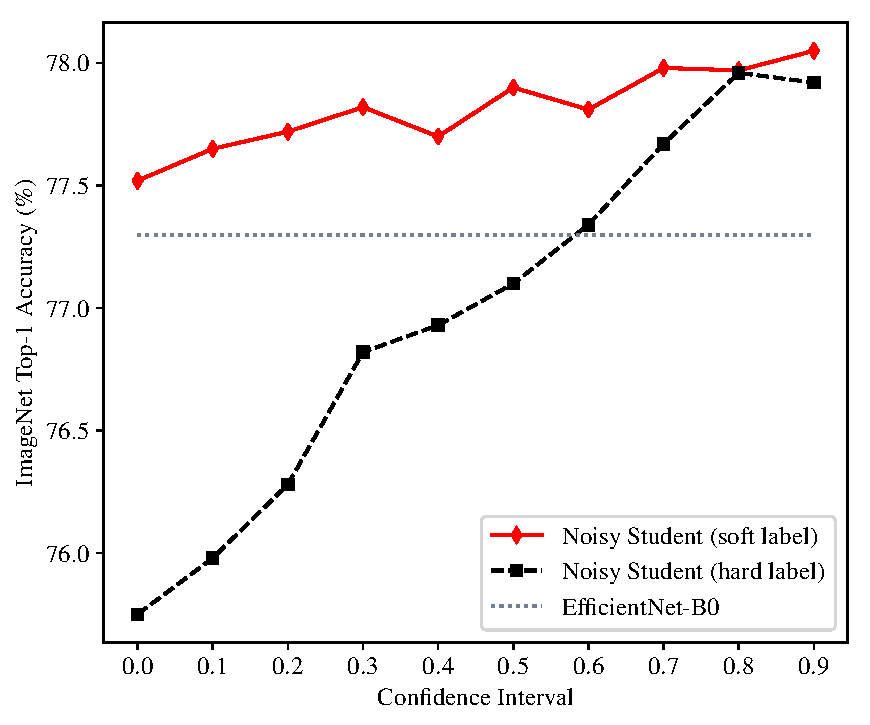
\includegraphics[width=0.9\columnwidth]{fig/plot_confidence.pdf}     \caption{对低自信度数据使用软性“假”标注会得到更好的结果。}  
	\label{fig:soft_vs_hard_vary_confidence} 
\end{figure}

\subsection{对未标注数据使用量的研究}
我们还对使用不同数量的未标注数据的效果进行了研究。我们从1.3亿未标注图像开始,逐步减少图像数量。为了简化实验,虽然选高自信度的图像会带来更好的结果,但是我们用均匀抽样(uniform sampling)的方法从整个数据集中抽取了$\frac{1}{128}, \frac{1}{64}, \frac{1}{32}, \frac{1}{16}, \frac{1}{4}$的图像。我们用EfficientNet-B4同时作为“学生”和“老师”。正如表\ref{tab:vary_unlabeled_data}中看到的那样,数据量减少到总数据量的$\frac{1}{16}$,也就是810万时(包括复制的图像),结果几乎保持不变。如果继续减少数据量,成绩开始下降。模型是否能够从更多的数据中受益取决于模型本身的容量,因为小的模型很容易饱和,而大的模型可以获益于更多数据。

\begin{table}[h!]
	\footnotesize
	\centering
	\begin{tabular}{c|cccccc}
		\toprule
		Data Reduction & $1/128$ & $1/64$ & $1/32$ & $1/16$ & $1/4$ & $1$ \\
		\midrule
		Top-1 Acc.  &83.4 & 83.3 & 83.7 & 83.9 & 83.8 & 84.0 \\
		\bottomrule
	\end{tabular}
	\caption{更多的未标注数据可以提高“吵闹学生”的表现。基准模型的准确率为83.2}
	\label{tab:vary_unlabeled_data}
\end{table}


\subsection{对“老师”模型容量的研究}
在前面所有的研究中,“学生”模型的容量都和“老师”模型相当或者更大。这里我们研究是否能够用一个更大的“老师”来提高一个小“学生”的成绩,因为小的模型在需要限制模型大小和延迟的现实情况中很有用。我们用我们最好的模型:“吵闹学生”法训练的EfficientNet-L2来训练从EfficientNet-B0到EfficientNet-B7的“学生”模型。为了简便,这里没有使用迭代训练。在这个实验中,我们用一般的数据扩增代替了RandAugment法。  


比较结果如表\ref{tab:vary_model_size}所示。用“吵闹学生”法训练的EfficientNet-L2作为“老师”可以把用“吵闹学生”法训练的模型的成绩再提升0.8\%左右。值得注意的是,和监督学习法相比,EfficientNet-B7的准确率提高了1.8\%.这表示,即使是需要用小的模型进行部署,用“吵闹学生”法先训练一个大的“老师”也是很有帮助的。

\begin{table}[h!]
	\centering
	\footnotesize
	\begin{tabular}{l|c|cc}
		\toprule
		Model & \# Params & Top-1 Acc. & Top-5 Acc. \\
		\midrule 
		EfficientNet-B0 & \multirow{3}{*}{5.3M} & 77.3 & 93.4  \\
		Noisy Student (B0) & & 78.1 & 94.2 \\
		\bf Noisy Student (B0, L2) & & \bf 79.0 & \bf 94.6\\
		\midrule
		EfficientNet-B1 & \multirow{3}{*}{7.8M} & 79.2 & 94.4  \\
		Noisy Student (B1) & & 80.3 & 95.1 \\
		\bf Noisy Student (B1, L2) & & \bf 81.4 & \bf 95.6 \\
		\midrule
		EfficientNet-B2 & \multirow{3}{*}{9.2M} & 80.0 & 94.9 \\
		Noisy Student (B2) & & 81.1 & 95.5 \\
		\bf Noisy Student (B2,  L2) & & \bf 82.2 & \bf 96.0 \\
		\midrule
		EfficientNet-B3 & \multirow{3}{*}{12M} & 81.7 & 95.7  \\
		Noisy Student (B3) & & 82.4 & 96.2 \\
		\bf Noisy Student (B3, L2) & & \bf 83.4  & \bf 96.6 \\
		\midrule
		EfficientNet-B4 & \multirow{3}{*}{19M} & 83.2 &  96.4 \\
		Noisy Student (B4) & & 84.0 & 96.8  \\
		\bf Noisy Student (B4, L2) & & \bf 84.9 & \bf 97.2 \\
		\midrule
		EfficientNet-B5 & \multirow{3}{*}{30M} & 84.0 & 96.8  \\
		Noisy Student (B5) & & 84.9  & 97.2 \\
		\bf Noisy Student (B5, L2) & & \bf 85.6 & \bf 97.6 \\
		\midrule
		EfficientNet-B6 & \multirow{3}{*}{43M} & 84.5 & 97.0  \\
		Noisy Student (B6) & & 85.3 & 97.5 \\
		\bf Noisy Student (B6, L2) & & \bf 86.0 & \bf 97.7 \\
		\midrule
		EfficientNet-B7 & \multirow{3}{*}{66M} & 85.0 & 97.2  \\
		Noisy Student (B7) & & 85.9 & 97.6 \\
		\bf Noisy Student (B7, L2) & & \bf 86.8 & \bf 98.0 \\
		\bottomrule
	\end{tabular}
	\caption{Noisy Student (B7)表示用EfficientNet-B7同时作为“老师”和“学生”模型。Noisy Student (B7, L2)表示用EfficientNet-B7做“学生”,用我们最好的准确率87.4\%的模型做“老师”。对于比“老师”小的“学生”模型,用我们最好的模型做“老师”所带来的提升比用同样架构的模型做“老师”带来的提升大。这说明即使需要使用小模型来做部署,用我们的方法来提高依旧可以提高}
	\label{tab:vary_model_size}
\end{table}

% \newpage
\subsection{健壮性基准测试中使用的指标的解释}
\paragraph{ImageNet-A} 
第一和前五准确率是基于ImageNet-A包含的200个类测量的。从这200个类到ImageNet原始类的映射可以在这里\footnote{https://github.com/hendrycks/natural-adv-examples/blob/master/eval.py}找到。

\paragraph{ImageNet-C}
mCE(平均损错误率,mean corruption error)是不同损毁方式中的错误率的加权平均,以AlexNet的错误率作为基线。分数都以AlexNet的错误率为标准进行归一化,这样不同难度的损毁方式下的分数都在相似的范围内。关于平均损毁错误率和AlexNet的错误率的详细解释请参考\cite{hendrycks2018benchmarking}。第一准确率就是简单的指所用损毁方式和所用严重程度下的平均第一准确率。

\paragraph{ImageNet-P} 
翻转率是指模型在不同干扰下改变第一预测的机率。mFR(平均翻转率,mean flip rate)是不同干扰下的翻转率的加权平均,以AlexNet的翻转率作为基线。关于平均翻转率和AlexNet的翻转率的详细解释请参考\cite{hendrycks2018benchmarking}。本文中第一准确率是指ImageNet-P包含的所有图像的准确率的平均值。

\end{document}

